\subsection{一元积分的几何应用}

	\begin{ti}
		求曲线 $y = x \sqrt{4x - x^{2}}$ 在 $[0,4]$ 上与 $x$ 轴所围图形绕 $y$ 轴旋转一周所得的旋转体的体积.
	\end{ti}

	\begin{ti}
		求曲线 $y = \sqrt{ x (1 - x)^{9} }$ 在 $[0,1]$ 上与 $x$ 轴所围图形绕 $x$ 轴旋转一周所得的旋转体的体积.
	\end{ti}

	\begin{ti}
		求曲线 $y = \sin^{4}x$ 在 $[0,\uppi]$ 上与 $x$ 轴所围图形绕 $y$ 轴旋转一周所得的旋转体的体积.
	\end{ti}

	\begin{ti}
		设 $a > 0$,$0 < b < 1$,由曲线 $y = \ee^{x}$,直线 $y = 1$ 与直线 $x = ab$ 所围平面区域的面积记为 $S_{1}$,由曲线 $y = \ee^{x}$,直线 $x = ab$ 与直线 $y = \ee^{a}$ 所围平面区域的面积记为 $S_{2}$,若 $S_{1} = S_{2}$,求 $\lim_{a \to 0^{+}} b$.
	\end{ti}

	\begin{ti}
		设 $O$ 为坐标原点,$A(1,0)$,$B(1,1)$,$C(0,1)$,记边长为 $1$ 的正方形 $OABC$ 内位于曲线 $y = x^{2} + t$($t$ 为实数)下方图形的面积为 $S(t)$.
		\begin{enumerate}
			\item 求 $S(t)$ 的表达式;
			\item $S(t)$ 在 $[-1,1]$ 上是否满足拉格朗日中值定理的条件,说明理由.
		\end{enumerate}
	\end{ti}

	\begin{ti}
		设曲线方程为 $y = \ee^{-x}(x \geq 0)$.
		\begin{enumerate}
			\item 曲线 $y = \ee^{-x}$,$x$ 轴,$y$ 轴和直线 $x = \xi(\xi > 0)$ 所围平面图形绕 $x$ 轴旋转一周,得旋转体,求此旋转体体积 $V(\xi)$,以及满足 $V(a) = \frac{1}{2} \lim_{\xi \to +\infty} V(\xi)$ 的 $a$ 值;
			\item 在此曲线上找一点,使过该点的切线与两个坐标轴所夹平面图形的面积最大,并求出该面积.
		\end{enumerate}
	\end{ti}

	\begin{ti}
		设 $n$ 为正整数,$A_{n}$ 是在第一象限内曲线 $y = n \cos nx$ 与该曲线在点 $\bigl( \frac{\uppi}{2n},0 \bigr)$ 处的切线所围成的平面图形的面积. 则\kuo.

		\twoch{$A_{n}$ 与 $n$ 有关}{$A_{n}$ 与 $n$ 无关}{无法判断}{以上结论都不正确}
	\end{ti}

	\begin{ti}
		\begin{enumerate}
			\item 如图~\ref{fig:1.3.1} 所示,设曲线 $L$ 具有如下性质:中间曲线 $y = 2x^{2}$ 上每一点 $P$ 都使得图中 $A$ 的面积等于 $B$ 的面积,求曲线 $L$ 的方程;
			\item 如图~\ref{fig:1.3.1} 所示,若让 $A,B$ 绕 $y$ 轴旋转一周所得的旋转体体积相等,求曲线 $L$ 的方程.
		\end{enumerate}
		\begin{figure}[htbp]
			\centering
			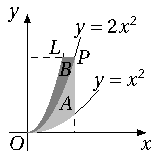
\includegraphics[scale=1]{figure/fig1-3-1.pdf}
			\caption{}\label{fig:1.3.1}
		\end{figure}
	\end{ti}

	\begin{ti}
		如图~\ref{fig:1.3.2} 所示,阴影部分由曲线 $y = \sin x(0 \leq x \leq \uppi)$,直线 $y = a(0 < a < 1)$,$x = \uppi$ 以及 $y$ 轴围成. 此图形绕直线 $y = a$ 旋转一周形成旋转体 $S$. 问 $a$ 为何值时,$S$ 有最小体积,$S$ 有最大体积.
		\begin{figure}[htbp]
			\centering
			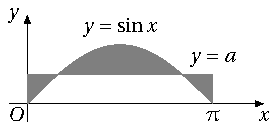
\includegraphics[scale=1]{figure/fig1-3-2.pdf}
			\caption{}\label{fig:1.3.2}
		\end{figure}
	\end{ti}

	\begin{ti}
		求曲线 $y^{2} = \bigl( 1 - x^{2} \bigr)^{3}$ 所围图形的面积.
	\end{ti}

	\begin{ti}
		求曲线 $\sqrt{x} + \sqrt{y} = 1$ 与坐标轴所围图形的面积.
	\end{ti}

	\begin{ti}
		求摆线 $x = t - \sin t$,$y = 1 - \cos t$ 的一拱与 $x$ 轴围成的图形的面积.
	\end{ti}

	\begin{ti}
		求星形线 $x = \cos^{3}t$,$y = \sin^{3}t$ 所围图形的面积.
	\end{ti}

	\begin{ti}
		求阿基米德螺线 $r = a \theta$ 的第一圈与极轴所围图形的面积.
	\end{ti}

	\begin{ti}
		求 $r = \sqrt{2} \sin \theta$ 及 $r^{2} = \cos 2 \theta$ 围成图形公共部分的面积.
	\end{ti}

	\begin{ti}
		求曲线 $y = \frac{1}{x^{2} + 1}$ 和 $x$ 轴之间区域的面积.
	\end{ti}

	\begin{ti}
		求曲线 $y = x \ee^{-\frac{x^{2}}{2}}$ 与其渐近线之间的面积.
	\end{ti}

	\begin{ti}
		记 $l_{1}$ 为椭圆 $x^{2} + 2y^{2} = 2$ 的周长,$l_{2}$ 为曲线 $y_{1} = \sin x$ 在 $0 \leq x \leq 2\uppi$ 上的弧长,$l_{3}$ 为曲线 $y_{2} = \frac{1}{2} \sin 2x$ 在 $0 \leq x \leq 2\uppi$ 上的弧长,则\kuo.

		\twoch{$l_{1} > l_{2} = l_{3}$}{$l_{1} = l_{2} < l_{3}$}{$l_{2} > l_{3} = l_{1}$}{$l_{1} = l_{2} = l_{3}$}
	\end{ti}

	\begin{ti}
		曲线 $\begin{cases}
			x = 3 (t - \sin t)\\
			y = 3 (1 - \cos t)
		\end{cases} (0 \leq t \leq 2\uppi)$ 的弧长为\htwo.
	\end{ti}

	\begin{ti}
		求抛物线 $6y = x^{2}$ 从点 $(0,0)$ 到点 $\bigl( 4,\frac{8}{3} \bigr)$ 之间的弧长.
	\end{ti}

	\begin{ti}
		求星形线 $x = \cos^{3}t$,$y = \sin^{3}t$ 的全长.
	\end{ti}

	\begin{ti}
		在摆线 $x = t - \sin t$,$y = 1 - \cos t$ 上求一点,将摆线第一拱的弧长分为 \ratio{$1$}{$3$}.
	\end{ti}

	\begin{ti}
		求心形线 $r = a (1 + \cos \theta)$ 的全长.
	\end{ti}

	\begin{ti}
		求曲线 $r \theta = 1$ 自 $\theta = \frac{3}{4}$ 至 $\theta = \frac{4}{3}$ 一段的弧长.
	\end{ti}

	\begin{ti}
		求曲线 $y = \int_{0}^{x} \sqrt{\cos t} \dd{t}$ 的全长.
	\end{ti}

	\begin{ti}
		当 $x \geq 0$ 时,曲线 $y = \frac{1}{4} \int_{0}^{2} x \sqrt{12 - x^{2} t^{2}} \dd{t}$ 的全长为\htwo.
	\end{ti}

	\begin{ti}
		设函数 $y = f(x)$ 在区间 $[0,1]$ 上非负、存在二阶导数,且 $f(0) = 0$,有一块质量均匀的平板 $D$,其占据的区域是曲线 $y = f(x)$ 与直线 $x = 1$ 以及 $x$ 轴围成的平面图形(图~\ref{fig:1.3.3}). 用 $\overline{x}$ 表示平板 $D$ 的质心的横坐标. 求证:
		\begin{enumerate}
			\item 若 $f'(x) > 0(0 \leq x \leq 1)$,则 $\overline{x} > \frac{1}{2}$(如图~\ref{fig:1.3.3:a});
			\item 若 $f''(x) > 0(0 \leq x \leq 1)$,则 $\overline{x} > \frac{2}{3}$(如图~\ref{fig:1.3.3:b}).
		\end{enumerate}
		\begin{figure}[htbp]
			\begin{floatrow}
			  \ffigbox[\textwidth]{
				\begin{subfloatrow}[2]
				  \ffigbox[\FBwidth]{
					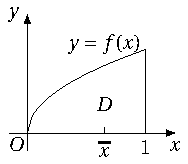
\includegraphics[scale=1]{figure/fig1-3-3-a.pdf}
				  }{\caption{}\label{fig:1.3.3:a}}
				  \ffigbox[\FBwidth]{
					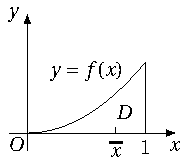
\includegraphics[scale=1]{figure/fig1-3-3-b.pdf}
				  }{\caption{}\label{fig:1.3.3:b}}
				\end{subfloatrow}
			  }{\caption{}\label{fig:1.3.3}}
			\end{floatrow}
		  \end{figure}
	\end{ti}

	\begin{ti}
		求由曲线 $y^{2} = x^{3} - x^{4}$ 所围成的平面图形的形心.
	\end{ti}

	\begin{ti}
		求由曲线 $y = x^{2}$ 与直线 $y = x$ 在第一象限内所围成的图形绕该直线旋转所成立体的体积.
	\end{ti}